\documentclass[border=4pt]{standalone}
\usepackage{amsmath,amssymb,amsfonts}
\usepackage{xcolor,colortbl,array,booktabs,multirow}
\usepackage{tikz}
\usepackage{pgfplots}
\pgfplotsset{compat=1.16}
\usetikzlibrary{arrows, automata, backgrounds, calendar, chains, decorations,
    matrix, mindmap, patterns, petri, positioning, shadows, shapes.geometric,
    trees, shapes, decorations.pathreplacing, calc, tikzmark, arrows.meta,
    intersections, fit, graphs, quotes, angles, decorations.markings}
\newcommand{\st}{\text{ s.t. }}
\newcommand{\x}{\mathbf{x}}
\renewcommand{\b}{\mathbf{b}}
\renewcommand{\c}{\mathbf{c}}
\newcommand{\A}{\mathbf{A}}
\newcommand{\y}{\mathbf{y}}
\newcommand{\z}{\mathbf{z}}
\newcommand{\R}{\mathbb{R}}
\newcommand{\RR}{\mathbb{R}}
\newcommand{\Z}{\mathbb{Z}}
\newcommand{\ZZ}{\mathbb{Z}}
\newcommand{\npcomplete}{NP-complete}
\providecommand{\true}{\text{TRUE}}
\providecommand{\false}{\text{FALSE}}
\tikzset{vertex/.style={circle,fill=black!25,minimum size=20pt,inner sep=0pt},
    edge/.style={draw,thick,-},weight/.style={font=\small},
    selected vertex/.style={vertex, fill=red!24},
    selected edge/.style={draw,line width=2pt,-,red!50},
    ignored edge/.style={draw,line width=2pt,-,black!20}}
\newcommand{\vect}{\vec}
\providecommand{\ds}{\displaystyle}
\providecommand{\longvect}{\overrightarrow}
\usepackage[normalem]{ulem}
\definecolor{ocre}{RGB}{243,102,25}
\providecommand{\leftB}{\left[}
\providecommand{\rightB}{\right]}
\tikzset{directed/.style={postaction={decorate,decoration={markings,mark=at position .65 with {\arrow{>}}}}},
    directed1/.style={postaction={decorate,decoration={markings,mark=at position .65 with {\arrow{>}}}}}}
\begin{document}
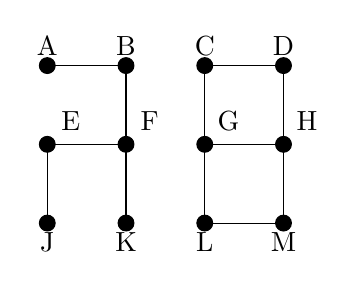
\begin{tikzpicture}
\draw[fill] (0,2) circle[radius=.1] node[above]{A};
\draw[fill] (1,2) circle[radius=.1] node[above]{B};
\draw[fill] (2,2) circle[radius=.1] node[above]{C};
\draw[fill] (3,2) circle[radius=.1] node[above]{D};
\draw[fill] (0,1) circle[radius=.1];
\node at (0.3,1.3){E}; 
\draw[fill] (1,1) circle[radius=.1];
\node at (1.3,1.3){F}; 
\draw[fill] (2,1) circle[radius=.1];
\node at (2.3,1.3){G};  
\draw[fill] (3,1) circle[radius=.1];
\node at (3.3,1.3){H};  
\draw[fill] (0,0) circle[radius=.1] node[below]{J};
\draw[fill] (1,0) circle[radius=.1] node[below]{K};
\draw[fill] (2,0) circle[radius=.1] node[below]{L};
\draw[fill] (3,0) circle[radius=.1] node[below]{M};
\draw(0,0)--(0,1);
\draw(1,0)--(1,1);
\draw(1,1)--(1,2);
\draw(2,0)--(2,1);
\draw(2,1)--(2,2);
\draw(3,0)--(3,1);
\draw(3,1)--(3,2);
\draw(2,0)--(3,0);
\draw(0,1)--(1,1);

\draw(2,1)--(3,1);
\draw(0,2)--(1,2);
\draw(2,2)--(3,2);
\end{tikzpicture}
\end{document}
